\begin{figure}[!t]
\centering
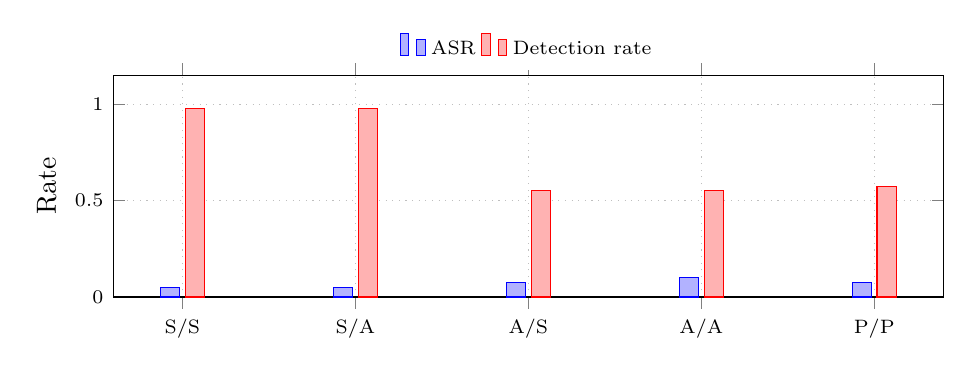
\begin{tikzpicture}
\begin{axis}[
  ybar,
  bar width=7pt,
  width=\columnwidth,
  height=4.4cm,
  ylabel={Rate},
  ymin=0, ymax=1.15,
  symbolic x coords={S/S, S/A, A/S, A/A, P/P},
  xtick=data,
  xticklabel style={font=\scriptsize},
  legend style={font=\scriptsize, at={(0.5,1.02)}, anchor=south, legend columns=2, draw=none},
  yticklabel style={font=\scriptsize},
  grid=major,
  major grid style={dotted,gray!50},
]
\addplot coordinates {(S/S,0.050) (S/A,0.050) (A/S,0.075) (A/A,0.100) (P/P,0.075)};
\addplot coordinates {(S/S,0.975) (S/A,0.975) (A/S,0.550) (A/A,0.550) (P/P,0.575)};
\legend{ASR, Detection rate}
\end{axis}
\end{tikzpicture}
\caption{Ladder outcomes. S\,=\,static, A\,=\,episodic adaptive,
P\,=\,persistent. Adaptive attackers cut detection from $0.975$ to
$0.55$.}
\label{fig:ladder}
\end{figure}
